\chapter{Simulations with Approximation Methods}
\label{chpt:app_sims}
Parts of this chapter has been published in \textcite{2020MNRAS.493.2085V}.
\section{Results for standard gravity}

\subsection{Simulation parameters}
We ran our simulations with the Planck \LCDM\ cosmology \parencite{planck_cosm}; its parameters are summarized in \autoref{tab:cosmo_param}. We expect our results to apply generically to cosmologies that are not too far from this set of parameter values.
\begin{table}
\begin{tabular}{ l c l }
  \hline \hline
  Hubble constant  [km s$^{-1}$ Mpc$^{-1}$] & $H_0$ & $67.74$ \\
  Baryon density parameter & $\Omega_b$ & $0.0486$ \\
  Matter density parameter & $\Omega_m$ & $0.3089$ \\
  Total density parameter & $\Omega_{tot}$ & $1$ \\
  Scalar spectral index & $n_s$ & $0.9667$ \\
  Fluctuation amplitude at $8\Mpch$ & $\sigma_8$ & $0.8159$ \\
  \hline \hline
\end{tabular}
\caption{Planck Collaboration cosmological parameters \parencite{planck_cosm} used in the simulations.}
\label{tab:cosmo_param}
\end{table}

In total, we ran and analyzed 7117 simulations using different approximations, parameters of the simulation volume and chameleon parameters. Their properties are described in \autoref{tab:sim_param_ZA_TZA} -- \autoref{tab:cham_param_CHI_nl}.

\begin{landscape}
\begin{table}
    \centering
    \adjustbox{max width=0.45\linewidth, max totalheight=0.9\textheight}{%
    \begin{tabular}{ ccccccc }
    \hline \hline
    $L$ & $N_{\rm p}$ & $N_{\rm f}$ & $N_{\rm a}$ & $N$ & $N_t$ & $m$ \\
    \hline
    $100$ & $512^3$ & $512^3$ & $1024^3$ & $1$ & $200$ & $9.4\cdot10^{8}$\\
    $100$ & $512^3$ & $512^3$ & $1024^3$ & $211$ & $100$ & $9.4\cdot10^{8}$\\
    $200$ & $512^3$ & $512^3$ & $1024^3$ & $1$ & $200$ & $7.6\cdot10^{9}$\\
    $200$ & $512^3$ & $512^3$ & $1024^3$ & $2$ & $100$ & $7.6\cdot10^{9}$\\
    $300$ & $512^3$ & $512^3$ & $1024^3$ & $1$ & $200$ & $2.6\cdot10^{10}$\\
    $400$ & $512^3$ & $512^3$ & $1024^3$ & $1$ & $200$ & $6.0\cdot10^{10}$\\
    $500$ & $512^3$ & $512^3$ & $1024^3$ & $1$ & $200$ & $1.2\cdot10^{11}$\\
    $500$ & $512^3$ & $512^3$ & $1024^3$ & $207$ & $100$ & $1.2\cdot10^{11}$\\
    $2000$ & $512^3$ & $512^3$ & $1024^3$ & $20$ & $400$ & $7.6\cdot10^{12}$\\
    $2000$ & $512^3$ & $512^3$ & $1024^3$ & $20$ & $200$ & $7.6\cdot10^{12}$\\
    $2000$ & $512^3$ & $512^3$ & $1024^3$ & $201$ & $100$ & $7.6\cdot10^{12}$\\
    $2000$ & $512^3$ & $512^3$ & $1024^3$ & $20$ & $50$ & $7.6\cdot10^{12}$\\
    $2000$ & $512^3$ & $512^3$ & $1024^3$ & $20$ & $25$ & $7.6\cdot10^{12}$\\
    \hline
    \end{tabular}
    }
    \hspace{2cm}
    \adjustbox{max width=0.45\linewidth, max totalheight=0.9\textheight}{%
    \begin{tabular}{ ccccccc }
    \hline \hline
    $L$ & $N_{\rm p}$ & $N_{\rm f}$ & $N_{\rm a}$ & $N$ & $N_t$ & $m$ \\
    \hline
    $100$ & $512^3$ & $512^3$ & $1024^3$ & $1$ & $200$ & $9.4\cdot10^{8}$\\
    $100$ & $512^3$ & $512^3$ & $1024^3$ & $100$ & $100$ & $9.4\cdot10^{8}$\\
    $100$ & $512^3$ & $512^3$ & $1024^3$ & $200$ & $100$ & $9.4\cdot10^{8}$\\
    $200$ & $512^3$ & $512^3$ & $1024^3$ & $1$ & $200$ & $7.6\cdot10^{9}$\\
    $200$ & $512^3$ & $512^3$ & $1024^3$ & $2$ & $100$ & $7.6\cdot10^{9}$\\
    $300$ & $512^3$ & $512^3$ & $1024^3$ & $1$ & $200$ & $2.6\cdot10^{10}$\\
    $400$ & $512^3$ & $512^3$ & $1024^3$ & $1$ & $200$ & $6.0\cdot10^{10}$\\
    $500$ & $512^3$ & $512^3$ & $1024^3$ & $1$ & $200$ & $1.2\cdot10^{11}$\\
    $500$ & $512^3$ & $512^3$ & $1024^3$ & $100$ & $100$ & $1.2\cdot10^{11}$\\
    $500$ & $512^3$ & $512^3$ & $1024^3$ & $201$ & $100$ & $1.2\cdot10^{11}$\\
    $2000$ & $512^3$ & $512^3$ & $1024^3$ & $20$ & $400$ & $7.6\cdot10^{12}$\\
    $2000$ & $512^3$ & $512^3$ & $1024^3$ & $20$ & $400$ & $7.6\cdot10^{12}$\\
    $2000$ & $512^3$ & $512^3$ & $1024^3$ & $20$ & $200$ & $7.6\cdot10^{12}$\\
    $2000$ & $512^3$ & $512^3$ & $1024^3$ & $20$ & $200$ & $7.6\cdot10^{12}$\\
    $2000$ & $512^3$ & $512^3$ & $1024^3$ & $99$ & $100$ & $7.6\cdot10^{12}$\\
    $2000$ & $512^3$ & $512^3$ & $1024^3$ & $201$ & $100$ & $7.6\cdot10^{12}$\\
    $2000$ & $512^3$ & $512^3$ & $1024^3$ & $20$ & $50$ & $7.6\cdot10^{12}$\\
    $2000$ & $512^3$ & $512^3$ & $1024^3$ & $20$ & $50$ & $7.6\cdot10^{12}$\\
    $2000$ & $512^3$ & $512^3$ & $1024^3$ & $20$ & $25$ & $7.6\cdot10^{12}$\\
    $2000$ & $512^3$ & $512^3$ & $1024^3$ & $20$ & $25$ & $7.6\cdot10^{12}$\\
    \hline
    \end{tabular}
    }
    \caption{Parameters of~the~simulations for~ZA (left) and~TZA (right): box size $L$ [$\Mpch$], number of~particles $N_{\rm p}$, number of~force mesh points $\Nf$, number of~power spectrum mesh points $N_{\rm a}$, number of~runs $N$, number of~time-steps $N_t$, and~a~derived parameter particle mass $m$ $[M_\odot]$.}
    \label{tab:sim_param_ZA_TZA}
    \end{table}
    
    
\begin{table}
    \centering
    \adjustbox{max width=0.45\linewidth, max totalheight=0.9\textheight}{%
    \begin{tabular}{ ccccccc }
    \hline \hline
    $L$ & $N_{\rm p}$ & $N_{\rm f}$ & $N_{\rm a}$ & $N$ & $N_t$ & $m$ \\
    \hline
    $2000$ & $64^3$ & $64^3$ & $128^3$ & $1$ & $100$ & $3.9\cdot10^{15}$\\
    $2000$ & $256^3$ & $256^3$ & $512^3$ & $99$ & $100$ & $6.0\cdot10^{13}$\\
    $100$ & $512^3$ & $512^3$ & $1024^3$ & $1$ & $200$ & $9.4\cdot10^{8}$\\
    $100$ & $512^3$ & $512^3$ & $1024^3$ & $211$ & $100$ & $9.4\cdot10^{8}$\\
    $200$ & $512^3$ & $512^3$ & $1024^3$ & $1$ & $200$ & $7.6\cdot10^{9}$\\
    $200$ & $512^3$ & $512^3$ & $1024^3$ & $2$ & $100$ & $7.6\cdot10^{9}$\\
    $300$ & $512^3$ & $512^3$ & $1024^3$ & $1$ & $200$ & $2.6\cdot10^{10}$\\
    $400$ & $512^3$ & $512^3$ & $1024^3$ & $1$ & $200$ & $6.0\cdot10^{10}$\\
    $500$ & $512^3$ & $512^3$ & $1024^3$ & $1$ & $200$ & $1.2\cdot10^{11}$\\
    $500$ & $512^3$ & $512^3$ & $1024^3$ & $208$ & $100$ & $1.2\cdot10^{11}$\\
    $2000$ & $512^3$ & $512^3$ & $1024^3$ & $20$ & $400$ & $7.6\cdot10^{12}$\\
    $2000$ & $512^3$ & $512^3$ & $1024^3$ & $20$ & $200$ & $7.6\cdot10^{12}$\\
    $2000$ & $512^3$ & $512^3$ & $1024^3$ & $201$ & $100$ & $7.6\cdot10^{12}$\\
    $2000$ & $512^3$ & $512^3$ & $1024^3$ & $20$ & $50$ & $7.6\cdot10^{12}$\\
    $2000$ & $512^3$ & $512^3$ & $1024^3$ & $19$ & $25$ & $7.6\cdot10^{12}$\\
    \hline
    \end{tabular}
    }
    \hspace{2cm}
    \adjustbox{max width=0.45\linewidth, max totalheight=0.9\textheight}{%
    \begin{tabular}{ ccccccc }
    \hline \hline
    $L$ & $N_{\rm p}$ & $N_{\rm f}$ & $N_{\rm a}$ & $N$ & $N_t$ & $m$ \\
    \hline
    $1000$ & $256^3$ & $256^3$ & $512^3$ & $303$ & $100$ & $7.6\cdot10^{12}$\\
    $2000$ & $256^3$ & $256^3$ & $512^3$ & $199$ & $100$ & $6.0\cdot10^{13}$\\
    $100$ & $512^3$ & $512^3$ & $1024^3$ & $1$ & $200$ & $9.4\cdot10^{8}$\\
    $100$ & $512^3$ & $512^3$ & $1024^3$ & $212$ & $100$ & $9.4\cdot10^{8}$\\
    $200$ & $512^3$ & $512^3$ & $1024^3$ & $1$ & $200$ & $7.6\cdot10^{9}$\\
    $200$ & $512^3$ & $512^3$ & $1024^3$ & $2$ & $100$ & $7.6\cdot10^{9}$\\
    $300$ & $512^3$ & $512^3$ & $1024^3$ & $1$ & $200$ & $2.6\cdot10^{10}$\\
    $400$ & $512^3$ & $512^3$ & $1024^3$ & $1$ & $200$ & $6.0\cdot10^{10}$\\
    $500$ & $512^3$ & $512^3$ & $1024^3$ & $1$ & $200$ & $1.2\cdot10^{11}$\\
    $500$ & $512^3$ & $512^3$ & $1024^3$ & $208$ & $100$ & $1.2\cdot10^{11}$\\
    $2000$ & $512^3$ & $512^3$ & $1024^3$ & $20$ & $400$ & $7.6\cdot10^{12}$\\
    $2000$ & $512^3$ & $512^3$ & $1024^3$ & $20$ & $200$ & $7.6\cdot10^{12}$\\
    $2000$ & $512^3$ & $512^3$ & $1024^3$ & $200$ & $100$ & $7.6\cdot10^{12}$\\
    $2000$ & $512^3$ & $512^3$ & $1024^3$ & $20$ & $50$ & $7.6\cdot10^{12}$\\
    $2000$ & $512^3$ & $512^3$ & $1024^3$ & $20$ & $25$ & $7.6\cdot10^{12}$\\
    \hline
    \end{tabular}
    }
    \caption{Parameters of~the~simulations for~FF (left) and~FP (right): box size $L$ [$\Mpch$], number of~particles $N_{\rm p}$, number of~force mesh points $\Nf$, number of~power spectrum mesh points $N_{\rm a}$, number of~runs $N$, number of~time-steps $N_t$, and~a~derived parameter particle mass $m$ $[M_\odot]$.}
    \label{tab:sim_param_FF_FP}
    \end{table}
    
    
    
\begin{table}
    \adjustbox{max width=0.45\linewidth, max totalheight=0.9\textheight}{%
    \begin{tabular}{ ccccccc cc}
    \hline \hline
    $L$ & $N_{\rm p}$ & $N_{\rm f}$ & $N_{\rm a}$ & $N$ & $N_t$ & $m$ & $\Phiscr$ & $n$ \\
    \hline
    $2000$ & $256^3$ & $256^3$ & $512^3$ & $100$ & $100$ & $6.0\cdot10^{13}$ & $1.0\cdot10^{-4}$ & $0.5$ \\
    $2000$ & $256^3$ & $256^3$ & $512^3$ & $96$ & $100$ & $6.0\cdot10^{13}$ & $1.0\cdot10^{-5}$ & $0.7$ \\
    $2000$ & $256^3$ & $256^3$ & $512^3$ & $98$ & $100$ & $6.0\cdot10^{13}$ & $1.0\cdot10^{-6}$ & $0.5$ \\
    $2000$ & $256^3$ & $256^3$ & $512^3$ & $97$ & $100$ & $6.0\cdot10^{13}$ & $1.0\cdot10^{-5}$ & $0.5$ \\
    $2000$ & $256^3$ & $256^3$ & $512^3$ & $99$ & $100$ & $6.0\cdot10^{13}$ & $1.0\cdot10^{-5}$ & $0.1$ \\
    \hline
    \end{tabular}
    }
    \hspace{1cm}
    \adjustbox{max width=0.45\linewidth, max totalheight=0.9\textheight}{%
    \begin{tabular}{ ccccccc cc}
    \hline \hline
    $L$ & $N_{\rm p}$ & $N_{\rm f}$ & $N_{\rm a}$ & $N$ & $N_t$ & $m$ & $\Phiscr$ & $n$ \\
    \hline
    $1000$ & $256^3$ & $256^3$ & $512^3$ & $101$ & $100$ & $7.6\cdot10^{12}$ & $1.0\cdot10^{-5}$ & $0.5$ \\
    $2000$ & $256^3$ & $256^3$ & $512^3$ & $100$ & $100$ & $6.0\cdot10^{13}$ & $1.0\cdot10^{-6}$ & $0.5$ \\
    $2000$ & $256^3$ & $256^3$ & $512^3$ & $99$ & $100$ & $6.0\cdot10^{13}$ & $1.0\cdot10^{-5}$ & $0.1$ \\
    $2000$ & $256^3$ & $256^3$ & $512^3$ & $120$ & $100$ & $6.0\cdot10^{13}$ & $1.0\cdot10^{-5}$ & $0.5$ \\
    $2000$ & $256^3$ & $256^3$ & $512^3$ & $100$ & $100$ & $6.0\cdot10^{13}$ & $1.0\cdot10^{-5}$ & $0.7$ \\
    $2000$ & $256^3$ & $256^3$ & $512^3$ & $100$ & $100$ & $6.0\cdot10^{13}$ & $1.0\cdot10^{-4}$ & $0.5$ \\
    $100$ & $512^3$ & $512^3$ & $1024^3$ & $100$ & $100$ & $9.4\cdot10^{8}$ & $1.0\cdot10^{-5}$ & $0.5$ \\
    $500$ & $512^3$ & $512^3$ & $1024^3$ & $100$ & $100$ & $1.2\cdot10^{11}$ & $1.0\cdot10^{-5}$ & $0.5$ \\
    \hline
    \end{tabular}
    }
    \caption{Parameters of the pseudo-linear chameleon simulation for FF (left) and FP (right): box size $L$ [$\Mpch$], number of particles $N_{\rm p}$, number of force mesh points $N_{
    m f}$, number of power spectrum mesh points $N_{\rm a}$, number of runs $N$, number of time-steps $N_t$, a derived parameter particle mass $m$ $[M_\odot]$, screening potential $\Phiscr$ and the chameleon power-law exponent $n$.}
    \label{tab:cham_param_CHI_lin}
    \end{table}
    
    
    \begin{table}
    \adjustbox{max width=0.45\linewidth, max totalheight=0.9\textheight}{%
    \begin{tabular}{ ccccccc cc}
    \hline \hline
    $L$ & $N_{\rm p}$ & $N_{\rm f}$ & $N_{\rm a}$ & $N$ & $N_t$ & $m$ & $\Phiscr$ & $n$ \\
    \hline
    $2000$ & $256^3$ & $256^3$ & $512^3$ & $100$ & $100$ & $6.0\cdot10^{13}$ & $1.0\cdot10^{-5}$ & $0.5$ \\
    $2000$ & $256^3$ & $256^3$ & $512^3$ & $99$ & $100$ & $6.0\cdot10^{13}$ & $1.0\cdot10^{-5}$ & $0.1$ \\
    $2000$ & $256^3$ & $256^3$ & $512^3$ & $99$ & $100$ & $6.0\cdot10^{13}$ & $1.0\cdot10^{-4}$ & $0.5$ \\
    $2000$ & $256^3$ & $256^3$ & $512^3$ & $100$ & $100$ & $6.0\cdot10^{13}$ & $1.0\cdot10^{-5}$ & $0.7$ \\
    $2000$ & $256^3$ & $256^3$ & $512^3$ & $99$ & $100$ & $6.0\cdot10^{13}$ & $1.0\cdot10^{-6}$ & $0.5$ \\
    \hline
    \end{tabular}
    }
    \hspace{1cm}
    \adjustbox{max width=0.45\linewidth, max totalheight=0.9\textheight}{%
    \begin{tabular}{ ccccccc cc}
    \hline \hline
    $L$ & $N_{\rm p}$ & $N_{\rm f}$ & $N_{\rm a}$ & $N$ & $N_t$ & $m$ & $\Phiscr$ & $n$ \\
    \hline
    $1000$ & $256^3$ & $256^3$ & $512^3$ & $77$ & $100$ & $7.6\cdot10^{12}$ & $1.0\cdot10^{-5}$ & $0.5$ \\
    $2000$ & $256^3$ & $256^3$ & $512^3$ & $96$ & $100$ & $6.0\cdot10^{13}$ & $1.0\cdot10^{-6}$ & $0.5$ \\
    $2000$ & $256^3$ & $256^3$ & $512^3$ & $100$ & $100$ & $6.0\cdot10^{13}$ & $1.0\cdot10^{-5}$ & $0.1$ \\
    $2000$ & $256^3$ & $256^3$ & $512^3$ & $102$ & $100$ & $6.0\cdot10^{13}$ & $1.0\cdot10^{-5}$ & $0.5$ \\
    $2000$ & $256^3$ & $256^3$ & $512^3$ & $99$ & $100$ & $6.0\cdot10^{13}$ & $1.0\cdot10^{-5}$ & $0.7$ \\
    $2000$ & $256^3$ & $256^3$ & $512^3$ & $99$ & $100$ & $6.0\cdot10^{13}$ & $1.0\cdot10^{-4}$ & $0.5$ \\
    $100$ & $512^3$ & $512^3$ & $1024^3$ & $100$ & $100$ & $9.4\cdot10^{8}$ & $1.0\cdot10^{-5}$ & $0.5$ \\
    $500$ & $512^3$ & $512^3$ & $1024^3$ & $98$ & $100$ & $1.2\cdot10^{11}$ & $1.0\cdot10^{-5}$ & $0.5$ \\
    \hline
    \end{tabular}
    }
    \caption{Parameters of the non-linear chameleon simulation for FF and FP: box size $L$ [$\Mpch$], number of particles $N_{\rm p}$, number of force mesh points $N_{
    m f}$, number of power spectrum mesh points $N_{\rm a}$, number of runs $N$, number of time-steps $N_t$, a derived parameter particle mass $m$ $[M_\odot]$, screening potential $\Phiscr$ and the chameleon power-law exponent $n$.}
    \label{tab:cham_param_CHI_nl}
    \end{table}
    
\end{landscape}

%%%%%%%%%%%%%%%%%%%%%%%
% Matter power spectrum
%%%%%%%%%%%%%%%%%%%%%%%
\subsection{Matter Power Spectrum}
\label{sec:pwr_spec}
The power spectrum is defined by equation~\eqref{eq:pk}. In \autoref{fig:pwr_spec_all} we show the power spectra $P(k)$ at redshift $z=0$ for the different approximation schemes. The gray areas represent variation across different realizations (different simulation runs). We see that on large (linear) scales all approximations reproduce the linear theory prediction (note that this is because the FFA and FFP results have been compensated for slower growth, as described below). On smaller scales, differences between the approximations become apparent. The ZA loses power compared to the linear power spectrum on these scales due to shell-crossing. In contrast, FFA and FPA do much better and can even partially simulate non-linear clustering.
% In \autoref{fig:pwr_spec_all}, we used the so-called \textit{effective time}, described in the following subsection, to study the differences in the \textit{shape} of power spectra between the individual approximations. In the following we will show that FFA and FPA actually have slower growth than linear theory.

\begin{figure}[hbt]
\centering
	\begin{subfigure}{0.9\textwidth}
        \includegraphicscustomlegend{simulations_approx/pwr_spec/pwr_spec}
	\end{subfigure}
	\begin{subfigure}{0.9\textwidth}
		\includegraphicscustom{simulations_approx/pwr_spec/pwr_spec}
	\end{subfigure}%
    \caption{Matter power spectrum $P(k)$ at redshift $z=0$ for different approximation schemes. Grey areas represent variations across different runs. Due to shell-crossing, ZA filters the power at higher $k$, falling below the linear power spectrum, whereas FFA and FPA retain some features of the full non-linear clustering.}
    \label{fig:pwr_spec_all}
\end{figure}

%%%%%%%%%%%%%%%%%%%%%%%%%%%%%%%%%%%%%%%%
%%%%%  -> power spectrum difference
%%%%%%%%%%%%%%%%%%%%%%%%%%%%%%%%%%%%%%%%
\subsubsection{Comparison with linear theory}
The relative differences between power spectra and the linear predictions at different redshifts are plotted in \autoref{fig:pwr_spec_diff}. By the linear prediction, in this case, is meant the initial power spectrum of the realization linearly evolved to the given epoch. The error bars once again represent variation across different realizations but individual differences are computed from the same realization of the power spectrum.
\begin{figure*}[!hbt]
\centering
	\begin{subfigure}{1.0\textwidth}
        \includegraphicscustomlegend{simulations_approx/pwr_spec/pwr_spec_diff_init_ZA}
	\end{subfigure}
	\begin{subfigure}{0.5\textwidth}
		\includegraphicscustom{simulations_approx/pwr_spec/pwr_spec_diff_emu}	
		\caption{\LCDM\ (nl)}	
	\end{subfigure}
	\begin{subfigure}{0.5\textwidth}
		\includegraphicscustom{simulations_approx/pwr_spec/pwr_spec_diff_init_ZA}
		\caption{Zel'dovich approximation}
	\end{subfigure}%
	\begin{subfigure}{0.5\textwidth}
		\includegraphicscustom{simulations_approx/pwr_spec/pwr_spec_diff_init_TZA}
		\caption{Truncated Zel'dovich approximation}
	\end{subfigure}
	\begin{subfigure}{0.5\textwidth}
		\includegraphicscustom{simulations_approx/pwr_spec/pwr_spec_diff_init_FF}
		\caption{Frozen-flow approximation}
	\end{subfigure}%
	\begin{subfigure}{0.5\textwidth}
		\includegraphicscustom{simulations_approx/pwr_spec/pwr_spec_diff_init_FP}
		\caption{Frozen-potential approximation}
	\end{subfigure}
	\caption{Relative differences between power spectra of approximations and the linear prediction at different redshifts. ZA predicts power spectra at large scales very well but fails on small scales at later times. FFA and FPA do not have this problem at small scales but the power spectrum grows more slowly across all scales. The (CosmicEmu) non-linear power spectrum is shown in the upper panel for comparison.}
	\label{fig:pwr_spec_diff}
\end{figure*}

The upper panel shows the non-linear power spectrum $P(k)$ generated by the CosmicEmu emulator \parencite{Heitmann:2015xma} for comparison purposes. The emulator predictions involve interpolations across results from a finite number of high-resolution simulations run with different cosmological parameters; the results are accurate at the level of a few percent.

As expected, the ZA predicts power spectra at large scales very well but fails on small scales at later times. In the case of FFA and FPA, the power spectrum growth is slower than linear theory predicts but, unlike ZA, this behavior is across all scales and there is significantly less suppression of power on smaller scales.

%%%%%%%%%%%%%%%%%%%%%%%
% Effective redshift
%%%%%%%%%%%%%%%%%%%%%%%
\subsection{Effective Redshift}
\label{sec:z_eff}
%%%%%%%%%%%%%%%%%%%%%%%%%%%%%%%%%%%%%%%%
%%%%%  -> suppression
%%%%%%%%%%%%%%%%%%%%%%%%%%%%%%%%%%%%%%%%
The power spectrum growth is slower than the linear prediction in the case of FFA or FPA. For FFA, this can be understood from the equation of motion \eqref{eq:FFA}. As the particles approach the minimum of the gravitational well, their velocities decrease as the gradient of the potential drops. In these approximations, as the velocity potential is constant in time, there is no change in slope as more and more particles arrive into the gravitational well, which is certainly not realistic. (If possible, the resulting artifacts should be corrected when using these approximations.)

For FPA, the reason for the suppression is very similar, although not as significant. Particles are not moving without any memory of their previous positions as in the case of FFA. They do not stop at the bottom of the well but rather oscillate around it. However, equation \eqref{eq:FPA} still drives them toward the velocities of FFA and they slow down inside gravitational wells.

Note that this effect of slower growth due to a decreasing gradient of the velocity potential is not bound to some particular scale -- it occurs both in shallow large wells as well as in deep and more concentrated wells. Consequently, it can be compensated via a correction factor. A similar situation occurs in particle-mesh codes when the number of time-steps is restricted because the assumption of constancy in velocity and force (the ``drift'' and ``kick'' terms in a standard integrator) fails to hold. In approximate particle-mesh codes, this error may be compensated by employing a ZA-motivated correction~(\cite{Ref:Feng}) in the time-stepping. The same technique could be applied here by combining the approximations in a suitable way or, as we do, by simply calibrating against linear theory, which yields the same result.

Additionally, the dynamical approximations in FFA and FPA can lead to artificial non--linear enhancement of the growth at later times on small scales within deep wells. It takes more time to get into a local gravitational well than in standard \nbody\ but once the particles are there, they may form stable cores as they simply move towards the local potential minimum. On these small scales, the approximations are not valid in any case, so this point is mostly academic.

As discussed above, the suppression of linear growth in FFA and FPA can be viewed as a modified growth function and we can introduce a simple rescaling via an effective redshift $z\eff$ so that the power spectrum on large linear scales matches the linear prediction
\eq{
	\langle P(k, z\eff) \rangle = \langle P\lin(k, z)\rangle\,,
}
where we are averaging over ``large scales''. In our simulations this mean we are fitting the linear power spectrum in the range from the minimum available wave-number $k_\text{\tiny min}=2\pi/L$ to half a decade $k=\sqrt{10}k_\text{\tiny min}$.

In the rest of the paper when we are comparing our results with a prediction of the linear or non--linear theory, we use this effective time instead of the simulation time unless stated otherwise.

In \autoref{fig:D_eff_Pk}, we compare the effective growth function with the linear growth function of \LCDM. For ZA and TZA there is almost no suppression as we are comparing large scales. However, at later times (or if we had used smaller scales) we would see an exponential suppression as described in \cite{Bharadwaj_1996}. For FFA and FPA we have an almost linear dependence of $D\eff$ on $a$, for FFA with a slope of approximately $8\%$ and for FPA with the slope being approximately $6\%$.
\begin{figure}[bt]
  \centering
    \begin{subfigure}{0.9\textwidth}
        \includegraphicscustomlegend{simulations_approx/z_eff/D_eff_Pk}
	\end{subfigure}
	\begin{subfigure}{0.9\textwidth}
        \includegraphicscustom{simulations_approx/z_eff/D_eff_Pk}
	\end{subfigure}
  \caption{Effective growth factor $D\eff$ for different approximation schemes based on ratio of power spectrum on large scales compared to the linear prediction.}
  \label{fig:D_eff_Pk}
\end{figure}

In \autoref{fig:timestep} we study the dependence of $D\eff$ on the number of time-steps. A larger number of time-steps improves $D\eff$ for FPA but, as expected, cannot eliminate the effect. In the case of FFA, $D\eff$ actually decreases with increase in number of time-steps. In this case, for smaller number of time-steps, particles do not evolve exactly along characteristic curves of the (initial) potential and the deceleration is suppressed.
\begin{figure}[bt]
  \centering
    \begin{subfigure}{0.9\textwidth}
        \includegraphicscustomlegend{simulations_approx/z_eff/timesteps}
	\end{subfigure}
	\begin{subfigure}{0.9\textwidth}
        \includegraphicscustom{simulations_approx/z_eff/timesteps}
	\end{subfigure}
  \caption{Effective growth factor $D\eff$ at $z=0$ for FFA and FPA as a function of number of time-steps.}
  \label{fig:timestep}
\end{figure}

After the linear theory compensation via the effective time, all approximations match the linear prediction on large scales (by definition), however, on smaller scales there are considerable differences. In the case of ZA (and TZA) at early times there is enhancement of power above linear theory, but at later times, the lack of the ability to follow small-scale structure (``diffusion'' at caustics) causes a suppression of power that continues to leak to larger scales. For FFA and FPA, however, the behavior is quite different. At early times particles on the smallest scales are almost in the minimum of the local gravitational potential (and consequently at the minimum of the velocity potential) and do not evolve much. This effect is weaker for FPA where particles have inertia and are not overdamped. At later times more and more particles end up in these (constant-in-time) gravitational wells and we observe (partial) non--linear gravitational clustering.


%%%%%%%%%%%%%%%%%%%%%%%
% Correlation function
%%%%%%%%%%%%%%%%%%%%%%%
\subsection{Correlation Function}
\label{sec:corr}
The two-point correlation function is defined as
\eq{
\label{eq:bao}
\xi(r)=\left\langle \delta(\mb x)\delta(\mb{x+r})\right\rangle=\int\frac{\dd^3\mb k}{(2\pi)^3}P(k)e^{i\mb{k\cdot r}}\,.
}
We computed the correlation function $\xi(r)$ for different approximation schemes at different redshifts directly from the measured matter power spectrum $P(k)$ using equation \eqref{eq:bao}. In \autoref{fig:corr_func}, we display an example of the correlation function at redshift $z=0.5$. All approximations agree reasonably with the full non-linear predictions of the emulator for the location of the BAO peak and its width.
\begin{figure}
\centering
	\begin{subfigure}{\textwidth}
        \includegraphicscustomlegend{simulations_approx/corr_func/corr_func_r2_z_z_eff}
	\end{subfigure}
	\begin{subfigure}{\textwidth}
		\centering
		\includegraphicscustom{simulations_approx/corr_func//corr_func_r2_z_z_eff}
	\end{subfigure}
	\caption{Two-point correlation function for different approximation schemes at $z=0.5$}.
	\label{fig:corr_func}
\end{figure}

Individual features of the BAO peak -- location $r_0$, amplitude $A$ and width $\sigma$ -- are obtained by fitting a Gaussian to $r^2\xi(r)$ around the BAO peak
\eq{
\xi_G(r)=A\cdot e^{-(r-r_0)^2/2\sigma^2}
}
In \autoref{fig:corr_peak}, we show the these features of the BAO peak relative to the non-linear predictions of the emulator as a function of time. All approximations can predict the location of the peak with 1\% accuracy. In predicting the shape of the peak, however, they do worse -- all approximations deviate in predictions for the peak width and amplitude. Note that which approximation does best (compared to the others) for a given quantity is a function of redshift.

%From comparison with the linear theory we see that FFA and FPA are predicting something between the linear and non-linear prediction but ZA and TZA predict values quite off the linear prediction as one would expect from these approximations.

\begin{figure}
\centering
	\begin{subfigure}{\textwidth}
        \includegraphicscustomlegend{simulations_approx/corr_func/corr_peak_loc_z_eff}
	\end{subfigure}
	\begin{subfigure}{\textwidth}
		\centering
		\includegraphicscustom{simulations_approx/corr_func//corr_peak_loc_z_eff}
		\caption{Location}
	\end{subfigure}
	\begin{subfigure}{\textwidth}
		\centering
		\includegraphicscustom{simulations_approx/corr_func//corr_peak_amp_z_eff}
		\caption{Amplitude}
	\end{subfigure}
	\begin{subfigure}{\textwidth}
		\centering
		\includegraphicscustom{simulations_approx/corr_func//corr_peak_width_z_eff}
		\caption{Width}
	\end{subfigure}
	\caption{Location, amplitude and width of the BAO peak (relative to the non-linear prediction) as a function of the redshift.}
	\label{fig:corr_peak}
\end{figure}

%%%%%%%%%%%%%%%%%%%%%%%
% Halo mass function
%%%%%%%%%%%%%%%%%%%%%%%
\subsection{Halo mass function}
In \autoref{fig:hmf_diff_z}
% \renewcommand{\zone}{3.9}
% \renewcommand{\ztwo}{1.8}
% \renewcommand{\zthree}{0.5}
% \renewcommand{\zfour}{0.0}
\begin{figure*}
	\centering
		\begin{subfigure}{1.0\textwidth}
			\includegraphicscustomlegend{simulations_approx/hmf/z0.0_b500_M1024_hmf_z_z_eff}
		\end{subfigure}
		\begin{subfigure}{0.5\textwidth}
			\includegraphicscustom{simulations_approx/hmf/z3.9_b500_M1024_hmf_z_z_eff}
			\caption{$z = $}
		\end{subfigure}%
		\begin{subfigure}{0.5\textwidth}
			\includegraphicscustom{simulations_approx/hmf/z1.8_b500_M1024_hmf_z_z_eff}
			\caption{$z = $}
		\end{subfigure}
		\begin{subfigure}{0.5\textwidth}
			\includegraphicscustom{simulations_approx/hmf/z0.5_b500_M1024_hmf_z_z_eff}
			\caption{$z = $}
		\end{subfigure}%
		\begin{subfigure}{0.5\textwidth}
			\includegraphicscustom{simulations_approx/hmf/z0.0_b500_M1024_hmf_z_z_eff}
			\caption{$z = $}
		\end{subfigure}
		\caption{Halo mass function for different approximation schemes at different redshifts.}
		\label{fig:hmf_diff_z}
	\end{figure*}



%%%%%%%%%%%%%%%%%%%%%%%
% Correlation function
%%%%%%%%%%%%%%%%%%%%%%%
\section{Results for modified gravity}
In this section we apply the approximate techniques to chameleon gravity (parameters as described in \autoref{tab:cham_param}), focusing on issues closely related to the scale where the chameleon field starts to affect the matter distribution. We first wish to study the effects of varying the simulation resolution on the power spectrum. Because the screening mechanism is directly related to the depth of the gravitational wells, and with lower spatial resolution, these wells are smeared, the role of resolution also needs to be understood. For this analysis we chose the FPA as this approximation is closest in spirit to \nbody s.

Following this, we compare the results of chameleon gravity directly against the FPA and FFA simulations. %These comparisons can tell us a lot about when and on what scales are chameleon effects visible and which approximation is better for studying modified gravity. 
We will study both $k-$space effects (power spectrum) and real-space effects (BAO peak in the correlation function). For chameleon gravity we ran all simulations twice -- once solving the non-linear Poisson equation \eqref{eq:cham_u} using the multigrid solver, and the second using the pseudo-linear prediction for the chameleon in $k-$space given by \eqref{eq:chi_lin_k} corrected by \eqref{eq:chi_bulk}.

%%%%%%%%%%%%%%%%%%%%%%%%%%%%%%%%%%%%%%%%
% Approximation methods in modified gravity
%%%%%%%%%%%%%%%%%%%%%%%%%%%%%%%%%%%%%%%%
\subsection{Approximation methods in modified gravity}
\todo{

The transformation from the Jordan frame to the Einstein frame introduces non-standard coupling of the chameleon field to standard matter. This results in a fifth force, given in the non-relativistic limit by
\eq{
	\label{eq:cham_force}
	\dddd{\mb u_{\chi}}{a} = -\frac{3\mu}{2a}\frac{\beta}{\Mpl}\mb{\nabla}\chi \,.
}
}

When applying the approximation methods described in \autoref{chpt:app_schemes} to the chameleon equations, we have three choices on how to arrive at an approximate solution:
\begin{enumerate}
\item \label{itm:lin_q} Purely linear prediction in $(\mb q, a)$-space, solution \eqref{eq:chi_lin_x}

\item \label{itm:lin_k} Purely linear prediction in $(\mb k, a)$-space, solution \eqref{eq:chi_lin_k}

\item \label{itm:nl_x} Non-linear prediction in $(\mb x, a)$-space, solution \eqref{eq:cham_u}
\end{enumerate}

Choice \ref{itm:lin_q} means that there is no computational overhead and we can simply take the chameleon force to be $2\beta^2a^{-2}$ of the gravitational one. This method clearly overestimates the chameleon force at early times when the chameleon's Compton wavelength is short. This is because the solution \eqref{eq:chi_lin_x} does not take into account the non-zero mass of the field.

A better choice is to use \ref{itm:lin_k} where the non-zero mass is incorporated. This solution adds relatively little computational overhead over normal gravity -- needing (at least) one Fourier transform and also extra storage. The overdensity $\delta(\mb k, a)$ is either the linearly evolved one, i.e. $\delta(\mb k, a) = D(a)\delta_0(\mb k)$, or we can compute $\delta$ at each time-step from the current positions of particles. This adds extra computation when assigning the mass of particles on the grid and one extra Fourier transform to get $\delta(\mb k, a)$. 
However, we cannot use \eqref{eq:chi_lin_k} blindly to get a solution in real space as this linear approximation breaks down inside massive objects where we would get a negative solution. This effect is similar to a usage of linear evolution for $\delta$ where we can end up with regions where $\delta<-1$. We need to check if the resulting chameleon field is positive and fix it where it is not. We use the screening regime value \eqref{eq:chi_bulk} to get a positive solution. We will refer to this prediction as pseudo-linear since it can address some effects of the screening mechanism.

The most expensive choice is \ref{itm:nl_x} where we must iteratively solve nonlinear equations. Unlike other methods this one can address the screening regime inside and near massive objects but at the cost of the most computational overhead.

%%%%%%%%%%%%%%%%%%%%%%%%%%%%%%%%%%%%%%%%
% Effect of simulation resolution
%%%%%%%%%%%%%%%%%%%%%%%%%%%%%%%%%%%%%%%%
\subsection{Effect of simulation resolution}
In order to study the effects of the simulation resolution, we define this resolution via the Nyquist wave-number $\knq$
\eq{
\knq=\frac{\pi N_f}{L}\,.
}
We wish to study two things in particular. The first is the minimum resolution needed to explore some particular scale, i.e., whether non-linear effects on smaller scales can affect larger scales. The second is to study the validity range of the pseudo-linear approximation of the chameleon field. We want to investigate on which scale this approximation breaks down and cannot be used even for generating approximate results.

In \autoref{fig:chi_res}, we see several chameleon simulations $(n=0.5,\ \Phiscr=10^{-5})$ with different resolution as described in \autoref{tab:cham_param}. We compared the resulting power spectra directly with FPA simulations with the same parameters (box size, number of particles, etc.). There are four sets of simulations with different resolutions (Nyquist frequencies), each one with a pseudo-linear prediction for the chameleon field and a non-linear result from the multigrid solver.

For lower resolution $(\knq = 0.4~\hMpc$ and $\knq = 0.8~\hMpc$), the pseudo-linear theory predicts higher amplitude of the power spectrum as it underestimates the screening effect on smaller scales. However, with higher resolution (and the ability to see deeper gravitational wells) this pseudo-linear prediction starts to overestimate the screening and suppress the power spectrum sooner than in the non-linear solver. It is because the correction to the solution \eqref{eq:chi_lin_k} suppress the chameleon force completely -- not only inside massive objects but near those as well. The non-linear solution predicts suppressed forces nearby these massive objects but not completely. The exact scale when this happens is dependent on the screening potential -- lower $\Phiscr$ means we need finer resolution to see deep gravitational wells where the chameleon is in the screening regime. For the choice of the screening potential as in \autoref{fig:chi_res} $(\Phiscr=10^{-5})$ this crossover where we cannot use the linear prediction happens at $k\sim2~\hMpc$. However, as FPA cannot fully resolve non-linear features on scales $k\gtrsim1~\hMpc$  we cannot take this scale exactly.

We can also see that even with higher resolution the power spectra on large and medium scales remain the same. This may suggest that the non-linear effects due to coupling of different wave-numbers are small. However, as these results are coming from a quasi-linear approximation we should be cautious about such a statement. We will further explore this resolution effects of the chameleon gravity using full \nbody s in the future.

\begin{figure}
  \centering
	\begin{subfigure}{1.0\textwidth}
        \includegraphicscustomlegend{simulations_approx/chi/chi_resolution_eff}
	\end{subfigure}
	\begin{subfigure}{1.0\textwidth}
		\includegraphicscustom{simulations_approx/chi/chi_resolution_eff}
	\end{subfigure}
  \caption{Ratio of the power spectrum of chameleon gravity to FPA with different resolutions of simulations. All simulations have $n=0.5,\ \Phiscr=10^{-5}$. Dotted lines show pseudo-linear prediction of the chameleon field whereas solid lines show results for the full non-linear multigrid solver for the chameleon field. Dashed vertical lines show locations of corresponding Nyquist frequencies.}
  \label{fig:chi_res}
\end{figure}

%%%%%%%%%%%%%%%%%%%%%%%%%%%%%%%%%%%%%%%%
% Matter power spectrum
%%%%%%%%%%%%%%%%%%%%%%%%%%%%%%%%%%%%%%%%
\subsection{Matter power spectrum}
We now turn to results for the matter power spectrum; \autoref{fig:pwr_spec_chi_fp} shows power spectra for different chameleon parameters for modified gravity simulations with FFA and FPA.

The FFA predicts an increased enhancement of the power spectrum compared to the FPA, unlike the corresponding situation for $\Lambda$CDM. This can be understood from how dynamics is treated within the FFA. In case of standard gravity, the velocity of a particle decreases steadily as it approaches a minimum of the gravitational potential. In the case of chameleon gravity, however, once the particle is close enough to the potential minimum such that the screening effect kicks in, the fifth force is abruptly cut off and the particle stops at the potential minimum. In the case of FPA, the particles retain their velocities inside the screened regions and the clustering effect, therefore, is not as strong.

\begin{figure*}
\centering
	\begin{subfigure}{1.0\textwidth}
        \includegraphicscustomlegend{simulations_approx/chi/fp_pwr_spec}
	\end{subfigure}
	\begin{subfigure}{0.5\textwidth}
		\includegraphicscustom{simulations_approx/chi/fp_pwr_spec}
	\end{subfigure}%
	\begin{subfigure}{0.5\textwidth}
		\includegraphicscustom{simulations_approx/chi/ff_pwr_spec}
	\end{subfigure}
	\begin{subfigure}{0.5\textwidth}
		\includegraphicscustom{simulations_approx/chi/fp_pwr_spec_ratio_nl}
	\end{subfigure}%
	\begin{subfigure}{0.5\textwidth}
		\includegraphicscustom{simulations_approx/chi/ff_pwr_spec_ratio_nl}
	\end{subfigure}
    \caption{Matter power spectrum $P(k)$ at redshift $z=0$ for different chameleon parameters. On the left are results using FPA whereas on the right results using FFA. Grey areas represent variations across different runs. Higher screening potential leads to greater enhancement of the power spectrum due to the fifth force.}
    \label{fig:pwr_spec_chi_fp}
\end{figure*}

In \autoref{fig:CHI_FP_diff}, we compare simulations with different chameleon parameters directly with FPA and FFA. For the values of the chosen screening potential $(\Phiscr=10^{-6}, 10^{-5}, 10^{-4})$ and a given resolution, the pseudo-linear prediction slightly underestimates the screening effect. The dependence of the enhancement of the power spectrum on chameleon parameters is according to our expectations. A lower value of the screening potential leads to a shorter Compton wavelength and greater effect of screening and therefore lower enhancement. Lower value of the chameleon power-law exponent leads to a longer Compton wavelength and higher screening potential $\Phiscra$ and therefore greater enhancement. We also again see that FFA predicts greater enhancement than FPA.

\begin{figure*}
  \centering
	\begin{subfigure}{0.5\textwidth}
        \includegraphicscustomlegend{simulations_approx/chi/chi_pwr_diff_256m_1p_512M_2000b}
	\end{subfigure}
	\begin{subfigure}{0.5\textwidth}
		\includegraphicscustom{simulations_approx/chi/chi_pwr_diff_256m_1p_512M_2000b}
	\end{subfigure}%
	\begin{subfigure}{0.5\textwidth}
		\includegraphicscustom{simulations_approx/chi/chi_ff_pwr_diff_256m_1p_512M_2000b}
	\end{subfigure}
  \caption{Ratio of the power spectrum of chameleon gravity to FPA (left) and FFA (right) with different chameleon parameters. Dotted lines show pseudo-linear prediction of the chameleon field whereas solid lines show results for the full non-linear multigrid solver.}
  \label{fig:CHI_FP_diff}
\end{figure*}

In \autoref{fig:CHI_FP_diff_lin_ratio} we show the ratio of the power spectrum using the full non-linear solver of the chameleon field to results using pseudo-linear predictions. The enhancement of the pseudo-linear prediction on scales $k\sim0.1~\Mpch$ is at percent level, while again somewhat stronger for FFA.

\begin{figure*}
  \centering
	\begin{subfigure}{0.5\textwidth}
        \includegraphicscustomlegend{simulations_approx/chi/chi_pwr_diff_256m_1p_512M_2000b_lin_ratio}
	\end{subfigure}
	\begin{subfigure}{0.5\textwidth}
		\includegraphicscustom{simulations_approx/chi/chi_pwr_diff_256m_1p_512M_2000b_lin_ratio}
	\end{subfigure}%
	\begin{subfigure}{0.5\textwidth}
		\includegraphicscustom{simulations_approx/chi/chi_ff_pwr_diff_256m_1p_512M_2000b_lin_ratio}
	\end{subfigure}
  \caption{Ratio of the power spectrum of chameleon gravity to pseudo-linear prediction using FPA (left) and FFA (right) with different chameleon parameters.}
  \label{fig:CHI_FP_diff_lin_ratio}
\end{figure*}
%%%%%%%%%%%%%%%%%%%%%%%%%%%%%%%%%%%%%%%%
% Linear scale
%%%%%%%%%%%%%%%%%%%%%%%%%%%%%%%%%%%%%%%%

In \autoref{fig:chi_pwr_diff_map}, we compare chameleon gravity to the FPA through the ratio of their power spectra for one set of chameleon parameters $(n=0.5,\ \Phiscr=10^{-5})$ as a function of time and scale. Here we can see comparison of a non-linear prediction as well as a comparison with the chameleon mass (at a given time). The chameleon mass is a very good indicator at which time and on what scales we should expect to see some effects of the fifth force. This can be used to improve speed of the simulations at early times, when chameleon effects are negligible.
\begin{figure}
	\centering
	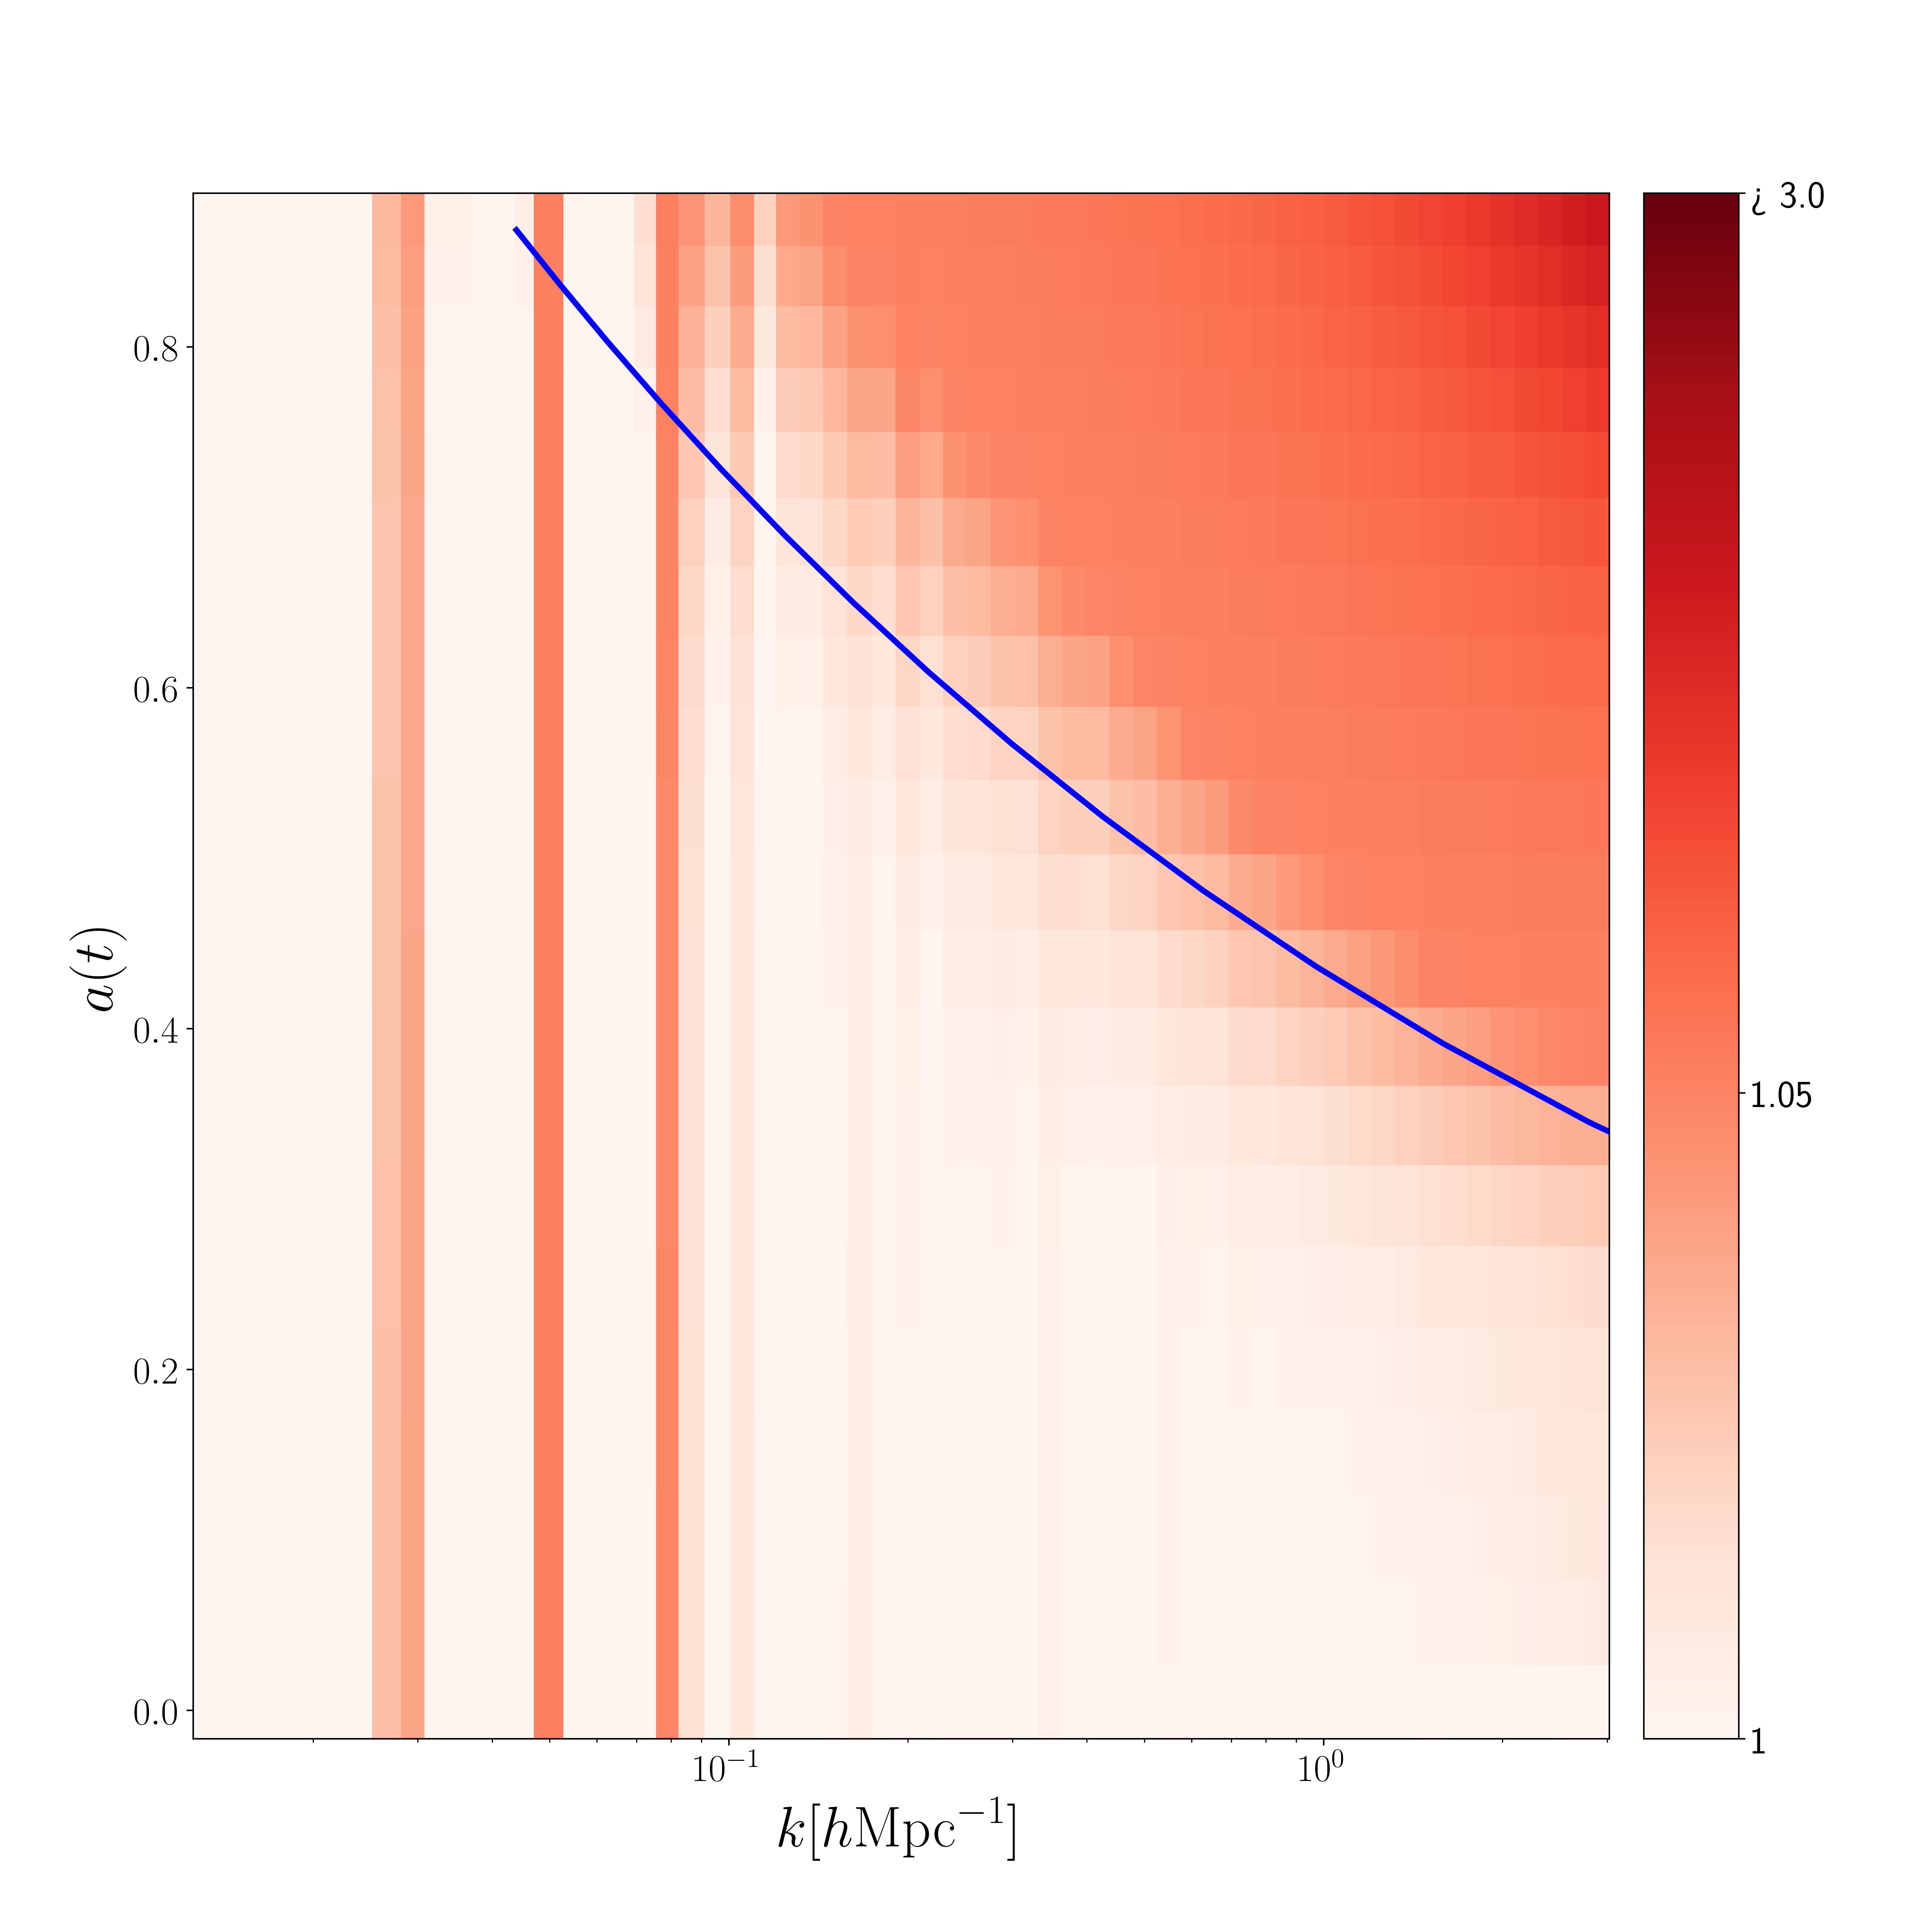
\includegraphics[width=1.0\linewidth]{simulations_approx/chi/chi_pwr_diff_map_512m_1p_1024M_500b_nl.png}
	\caption{Ratio of the FPA power spectrum in chameleon gravity $(n=0.5,\ \Phiscr=10^{-5})$ to the simulation run with standard gravity as function of time. Blue solid line is a chameleon mass \eqref{eq:chi_m}.}
	\label{fig:chi_pwr_diff_map}
\end{figure}

%%%%%%%%%%%%%%%%%%%%%%%%%%%%%%%%%%%%%%%%
% Correlation function
%%%%%%%%%%%%%%%%%%%%%%%%%%%%%%%%%%%%%%%%
\subsection{Correlation function}
In \autoref{fig:chi_corr_func}, we display the correlation function for one particular case of chameleon gravity -- $n=0.5,\ \Phiscr=10^{-5}$ at $z=0.5$. In \autoref{fig:chi_corr_peak}, we show the effects of different parameters of chameleon gravity through the BAO peak (amplitude, location and width). In this plot, the BAO peak characteristics are shown relative to the non-linear prediction (at the effective time) from the emulator. Comparison is done both for FPA (left) and FFA (right). We see that chameleon generally leads to a higher amplitude of the peak, a slight shift to the higher $r$ and a narrower width of the peak. All these effects are stronger for FFA than for FPA (as expected).

\begin{figure*}
\centering
	\begin{subfigure}{1.0\textwidth}
        \includegraphicscustomlegend{simulations_approx/chi/chi_corr_func_r2_z_z_eff}
	\end{subfigure}
	\begin{subfigure}{1.0\textwidth}
		\centering
		\includegraphicscustom{simulations_approx/chi/chi_corr_func_r2_z_z_eff}
	\end{subfigure}
	\begin{subfigure}{1.0\textwidth}
		\centering
		\includegraphicscustom{simulations_approx/chi/chi_ff_corr_func_r2_z_z_eff}
	\end{subfigure}
	\caption{Correlation function for chameleon gravity $(n=0.5,\ \Phiscr=10^{-5})$ at $z=0.5$. On the top are shown results using FPA whereas on the bottom using FFA}
	\label{fig:chi_corr_func}
\end{figure*}

\begin{figure*}
\centering
%%%%%%%%%%%%%%%%%%%%%%%%%%%%%%%%%%%%%
% Legend
%%%%%%%%%%%%%%%%%%%%%%%%%%%%%%%%%%%%%
	\begin{subfigure}{0.5\textwidth}
        \includegraphicscustomlegend{simulations_approx/chi/nl_fp_corr_peak_amp_z_eff}
	\end{subfigure}
%%%%%%%%%%%%%%%%%%%%%%%%%%%%%%%%%%%%%
% Amplitude
%%%%%%%%%%%%%%%%%%%%%%%%%%%%%%%%%%%%%
	\begin{subfigure}{0.5\textwidth}
		\includegraphicscustom{simulations_approx/chi/nl_fp_corr_peak_amp_z_eff}
		\caption{Amplitude}
	\end{subfigure}%
	\begin{subfigure}{0.5\textwidth}
		\includegraphicscustom{simulations_approx/chi/nl_ff_corr_peak_amp_z_eff}
		\caption{Amplitude}
	\end{subfigure}
%%%%%%%%%%%%%%%%%%%%%%%%%%%%%%%%%%%%%
% Loation
%%%%%%%%%%%%%%%%%%%%%%%%%%%%%%%%%%%%%
	\begin{subfigure}{0.5\textwidth}
		\includegraphicscustom{simulations_approx/chi/nl_fp_corr_peak_loc_z_eff}
		\caption{Location}
	\end{subfigure}%
	\begin{subfigure}{0.5\textwidth}
		\includegraphicscustom{simulations_approx/chi/nl_ff_corr_peak_loc_z_eff}
		\caption{Location}
	\end{subfigure}
%%%%%%%%%%%%%%%%%%%%%%%%%%%%%%%%%%%%%
% Width
%%%%%%%%%%%%%%%%%%%%%%%%%%%%%%%%%%%%%
	\begin{subfigure}{0.5\textwidth}
		\includegraphicscustom{simulations_approx/chi/nl_fp_corr_peak_width_z_eff}
		\caption{Width}
	\end{subfigure}%
	\begin{subfigure}{0.5\textwidth}
		\includegraphicscustom{simulations_approx/chi/nl_ff_corr_peak_width_z_eff}
		\caption{Width}
	\end{subfigure}
%%%%%%%%%%%%%%%%%%%%%%%%%%%%%%%%%%%%%
% Caption
%%%%%%%%%%%%%%%%%%%%%%%%%%%%%%%%%%%%%
	\caption{Location, amplitude and width of the BAO peak as a function of the redshift for different values of chameleon parameters. On the left, the characteristics are shown for simulations using FPA, while on the right, for simulations using FFA.}
	\label{fig:chi_corr_peak}
\end{figure*}

%%%%%%%%%%%%%%%%%%%%%%%%%%%%%%%%%%%%%%%%
% Halo mass function
%%%%%%%%%%%%%%%%%%%%%%%%%%%%%%%%%%%%%%%%
\subsection{Halo mass function}
